\documentclass{article}
\usepackage[utf8]{inputenc}
\usepackage{amsmath}
\usepackage{graphicx}
\usepackage{hyperref}
\usepackage{geometry}
\geometry{a4paper, margin=1in}

\title{Perishable Inventory Control with Shelf-Life Constraints\\ \large Reinforcement Learning Final Project}
\author{}
\date{}

\begin{document}

\maketitle

\section{Motivation}
Managing perishable inventory is a ubiquitous challenge across industries such as retail, healthcare (blood banks), and food distribution. This problem is particularly difficult due to \textbf{delayed consequences}: an order placed today will age over time, leading to potential waste if demand remains persistently low, or stockouts if demand unexpectedly surges. Traditional control policies (such as static base-stock levels) often struggle to balance the trade-off. 
Reinforcement Learning (RL) provides an elegant framework to learn intelligent inventory replenishment strategies from experience, specifically minimizing the dual risks of costly stockouts and excessive waste.

\section{Environment Description}
The problem is modeled as a Markov Decision Process (MDP) utilizing a First-Expire-First-Out (FEFO) issuing policy. 
\begin{itemize}
    \item \textbf{State Space ($\mathcal{S}$):} 
    The state is represented by a vector $S = (n_1, n_2, \dots, n_D)$, where $D$ is the maximum shelf-life. Each element $n_i$ represents the number of units in inventory with exactly $i$ days of shelf-life remaining.
    
    \item \textbf{Action Space ($\mathcal{A}$):} 
    The action $a \in \{0, 1, \dots, A_{\max}\}$ represents the discrete quantity of new inventory ordered at the beginning of the time step.
    
    \item \textbf{Transitions and Dynamics:} 
    A single time step progresses as follows:
    \begin{enumerate}
        \item \textbf{Receive:} New units $a$ are added to the freshest bucket (bucket $D$).
        \item \textbf{Demand:} A stochastic demand $d \sim \text{Poisson}(\lambda)$ is realized.
        \item \textbf{Sell (FEFO):} Demand is fulfilled by continually depleting the oldest available inventory (starting from $n_1$ towards $n_D$) until either demand is met or all stock is depleted.
        \item \textbf{Waste:} Any units remaining in bucket $1$ (0 days left) spoil and are discarded.
        \item \textbf{Age:} The remaining inventory ages by one day, shifting $n_{i} \leftarrow n_{i+1}$, and leaving bucket $D$ initially empty for the next step.
    \end{enumerate}
    
    \item \textbf{Reward Function ($\mathcal{R}$):} 
    The reward maps state transitions to numeric outcomes corresponding to profitability:
    \begin{equation}
        R(s, a) = p \cdot (\text{sold}) - c \cdot (\text{ordered}) - w \cdot (\text{wasted}) - s \cdot (\text{stockout})
    \end{equation}
    where $p$ is the selling price, $c$ is the ordering cost, $w$ is the waste penalty, and $s$ is the stockout penalty.
\end{itemize}

\section{Implemented Agents}
We approached the MDP using classical Dynamic Programming and diverse Reinforcement Learning algorithms:
\begin{itemize}
    \item \textbf{Dynamic Programming (Value Iteration):} Used as our optimal baseline. It iteratively computes the exact state-value function using the known transition dynamics and Poisson probabilities.
    \item \textbf{SARSA:} An on-policy temporal difference learning algorithm. It updates Q-values iteratively by following an $\epsilon$-greedy exploratory policy.
    \item \textbf{Q-Learning:} An off-policy temporal difference algorithm that learns the optimal policy directly by always bootstrapping from the maximum Q-value of the next state.
    \item \textbf{Monte Carlo (MC) Control:} It learns from full episodic returns rather than bootstrapping. We used first-visit MC with an $\epsilon$-greedy policy.
    \item \textbf{Linear Function Approximation (Linear FA):} An agent utilizing linear function approximation with extracted features rather than a tabular Q-function. It relies on a weight vector to generalize over the large state space.
\end{itemize}

\section{Results and Discussion}
The algorithms were trained and evaluated over 100 episodes. The results showcase distinct differences in learning stability, reward optimization, and operational trade-offs.

\subsection{Performance and Comparison}
\begin{itemize}
    \item \textbf{DP (Baseline):} As expected, the exact Value Iteration agent yielded the highest mean reward of 1295.10 across 100 test episodes, exhibiting minimal waste (0.24\%) and a steady fill rate of 83.5\%.
    \item \textbf{SARSA and Q-Learning:} Both tabular TD methods performed admirably. SARSA achieved a mean reward of 1243.02, closely tracking the DP bounds, while Q-learning settled slightly lower at 1148.68. SARSA's on-policy nature appeared to encourage a marginally safer, more robust tracking behavior in this specific hyperparameter setting.
    \item \textbf{Monte Carlo:} MC failed to learn a performant policy in the given timeframe, suffering massive stockouts (83.2\% stockout rate) and achieving a dramatically negative mean reward (-2022.60). Without bootstrapping, the credit assignment over the long delayed consequences of inventory proved overly sample-inefficient.
    \item \textbf{Linear FA:} Achieved an average reward of -311.92. While better than MC, the simple linear features failed to accurately capture the non-linear intricacies of the FEFO depletion logic across multiple shelf-life buckets, resulting in frequent stockouts (48.6\%).
\end{itemize}

\subsection{Visualizing the Trade-offs}
\begin{figure}[h]
    \centering
    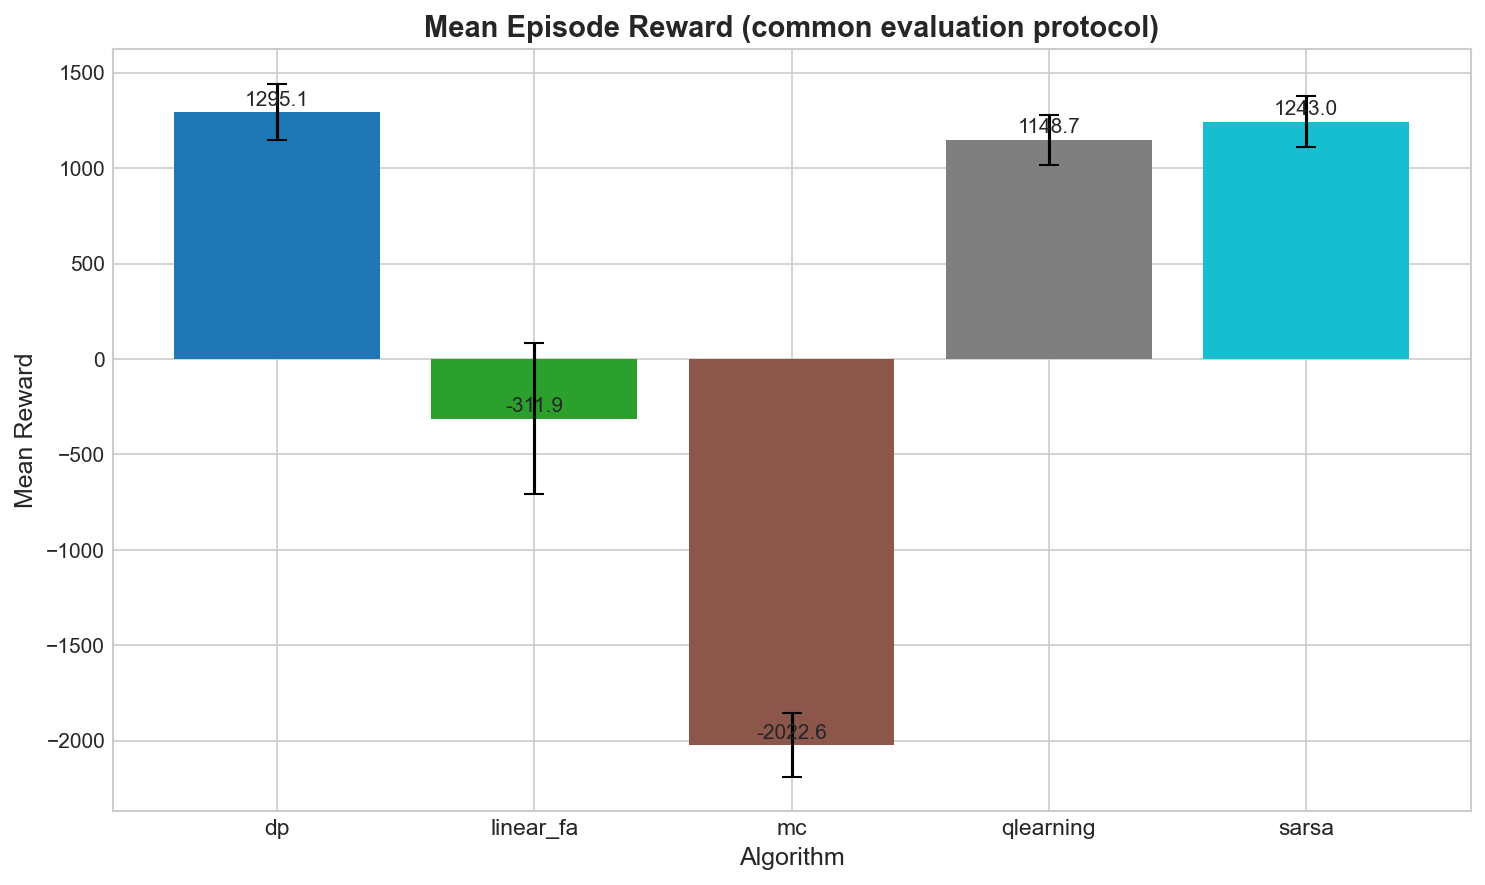
\includegraphics[width=0.7\textwidth]{outputs/figures/bar_reward_comparison.png}
    \caption{Mean reward comparison across all implemented formulations.}
\end{figure}

\begin{figure}[h]
    \centering
    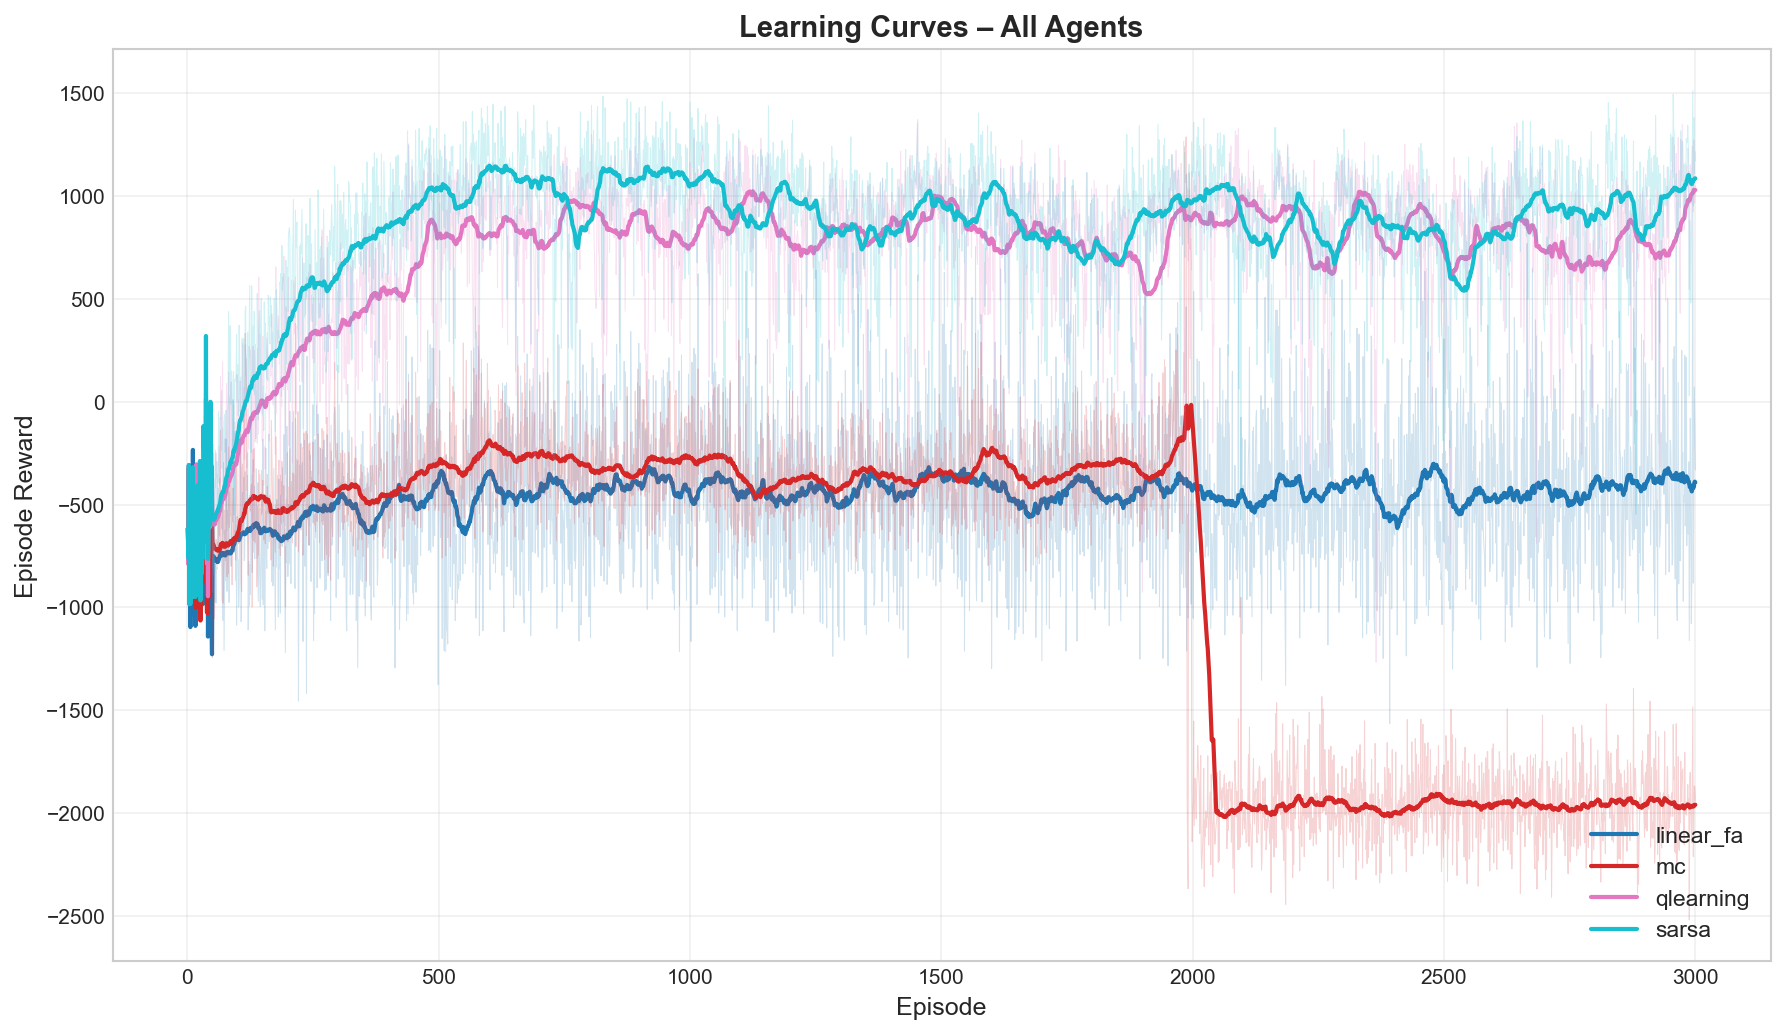
\includegraphics[width=0.7\textwidth]{outputs/figures/learning_curves_comparison.png}
    \caption{Learning stability and convergence across RL algorithms.}
\end{figure}

Visualizing the learning curves (\textit{learning\_curves\_comparison.png}) highlights how rapidly SARSA and Q-learning escape the initial negative-reward exploratory phases whereas Linear FA and MC struggle to isolate the optimal reorder triggers. Furthermore, the waste-stockout tradeoff plot clearly dictates that learning a balanced approach is key: highly aggressive order strategies risk massive waste penalties, while conservative policies suffer intense stockout costs. Only Tabular TD methods and DP reliably found the equilibrium.

\begin{thebibliography}{9}
\bibitem{sutton2018}
R. S. Sutton and A. G. Barto. \textit{Reinforcement Learning: An Introduction}. MIT press, 2018.

\bibitem{puterman2014}
M. L. Puterman. \textit{Markov Decision Processes: Discrete Stochastic Dynamic Programming}. John Wiley \& Sons, 2014.

\bibitem{nahmias1982}
S. Nahmias. ``Perishable Inventory Theory: A Review''. \textit{Operations Research}, 30(4):680--708, 1982.
\end{thebibliography}

\end{document}